\documentclass[11pt,letterpaper]{article}
\usepackage[margin=0.85in,headheight=14pt]{geometry}
\usepackage{amsmath,amssymb}
\usepackage{enumitem}
\usepackage{fancyhdr}
\usepackage{lmodern}
\usepackage[T1]{fontenc}
\usepackage[dvipsnames]{xcolor}
\usepackage[most]{tcolorbox}
\usepackage{listings}
\usepackage{pgfplots}
\usepgfplotslibrary{groupplots,fillbetween}
\usetikzlibrary{arrows.meta,positioning,shapes.geometric}
\pgfplotsset{
  compat=1.18,
  every axis/.append style={grid=major, grid style={gray!25}, tick label style={font=\footnotesize},
    label style={font=\small}, title style={font=\small}, legend style={font=\scriptsize}},
}
\definecolor{cA}{HTML}{1F77B4}
\definecolor{cB}{HTML}{FF7F0E}
\definecolor{cC}{HTML}{2CA02C}
\definecolor{cD}{HTML}{D62728}
\definecolor{cE}{HTML}{9467BD}

\pagestyle{fancy}
\fancyhf{}
\lhead{SYDE 556/750 \qquad Ramp practice}
\rhead{Solutions}
\cfoot{\thepage}
\renewcommand{\headrulewidth}{0pt}

\setlength{\parindent}{0pt}
\setlength{\parskip}{4pt}

\newcommand{\T}{\mathsf{T}}
\newcommand{\Jb}{J^{\mathrm{bias}}}
\newcommand{\tref}{\tau_{\mathrm{ref}}}
\newcommand{\trc}{\tau_{RC}}
\newcommand{\tin}{\tau_{\mathrm{in}}}
\newcommand{\ans}[1]{\par\vspace{4pt}{\bfseries #1}\quad}

\newtcolorbox{result}{colback=Green!6,colframe=Green!50!black,boxrule=0.5pt,left=4pt,right=4pt,top=2pt,bottom=2pt,arc=1pt}
\newtcolorbox{trap}{colback=red!4,colframe=red!50!black,boxrule=0.4pt,left=4pt,right=4pt,top=2pt,bottom=2pt,arc=1pt,fonttitle=\bfseries\small,title=Where marks are usually lost}

\lstset{basicstyle=\ttfamily\small, columns=fullflexible, keepspaces=true, frame=single, rulecolor=\color{gray!50}}

\begin{document}

\begin{center}
{\Large\bfseries Ramp practice solutions}\\[2pt]
{\large Nengo ensembles, vector transformations, and recurrent dynamics}\\[4pt]
Open a solution only after attempting that question. Each green box is the result.
\end{center}

%=====================================================================
\part*{Part A}
%=====================================================================

\section{The LIF tuning curve and its two time constants}

\ans{Q1}
\[
G(2) = \frac{1}{\tref - \trc\ln(1 - \tfrac12)} = \frac{1}{0.002 + 0.02\ln 2} \approx \frac{1}{0.0159} \approx 63\ \mathrm{Hz}.
\]
As $J \to \infty$, $\ln(1 - 1/J) \to 0$, so $G \to 1/\tref = 500\ \mathrm{Hz}$. The neuron can never fire faster than once per refractory period.

With $\tref = 5\,\mathrm{ms}$ the ceiling is $1/\tref = 200\ \mathrm{Hz}$. A neuron asked for $200\ \mathrm{Hz}$ would need infinite current, and anything above it is impossible. Nengo cannot find a finite gain, so the build fails or the gain blows up. Every maximum rate must satisfy $a^{\max} < 1/\tref$.
\begin{result}
$G(2) = 1/(0.002 + 0.02\ln 2) \approx 63$ Hz. Ceiling $1/\tref = 500$ Hz. At $\tref = 5$ ms the ceiling equals the requested $200$ Hz, which is unreachable.
\end{result}

\ans{Q2}
Nengo pins the curve at the intercept ($J = 1$ at $x = 0$) and at the maximum ($G = 200$ at $x = 1$). Solving $G(J^{\max}) = a^{\max}$:
\[
\tref - \trc\ln(1 - 1/J^{\max}) = \frac{1}{a^{\max}} \quad\Longrightarrow\quad J^{\max} = \frac{1}{1 - e^{(\tref - 1/a^{\max})/\trc}},
\qquad J(x) = 1 + (J^{\max} - 1)\,x.
\]
At $200$ Hz the inter-spike interval at the maximum is $5$ ms. With $\tref = 4$ ms, only $1$ ms of that is charging time, so the neuron at $x = 1$ is already pressed against its $250$ Hz ceiling. Its curve shoots up just above threshold and then flattens (very concave). With $\tref = 1$ ms there is $4$ ms of charging time, the ceiling of $1000$ Hz is far away, and the curve is closer to a straight line.

For $\trc$: the charging time $-\trc\ln(1 - 1/J)$ behaves like $\trc/J$ far above threshold, so the rate there is roughly linear in $J$. A large $\trc$ ($100$ ms) needs $J^{\max} \approx 34$ to reach $200$ Hz, so most of the range is far above threshold and nearly linear. A small $\trc$ ($10$ ms) reaches $200$ Hz already at $J^{\max} \approx 3.9$, so the whole curve sits in the sharply bending region near threshold.

More curvature means a sum of tuning curves approximates the straight line $x$ less well, so the RMSE is larger. Nengo, for 100 neurons: RMSE $0.0053$ at $\tref = 1$ ms and $0.0069$ at $4$ ms; $0.0074$ at $\trc = 10$ ms and $0.0036$ at $100$ ms.
\begin{center}
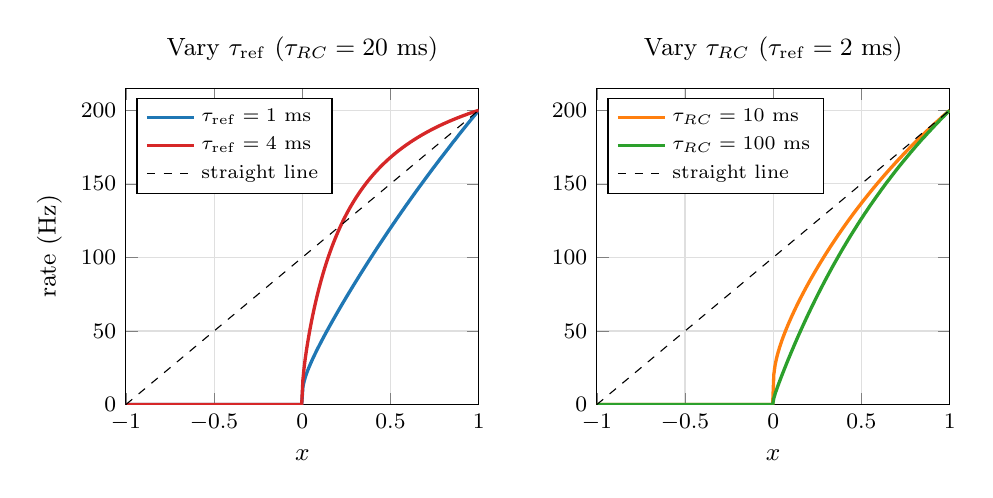
\begin{tikzpicture}[
  declare function={lif(\x,\tr,\tc,\Jm) = (\x > 0) * 1/(\tr - \tc*ln(1 - 1/(1 + (\Jm-1)*max(\x,1e-6))));}]
\begin{groupplot}[group style={group size=2 by 1, horizontal sep=1.5cm},
  width=0.5\textwidth, height=5.6cm, xmin=-1, xmax=1, ymin=0, ymax=215, xlabel={$x$},
  legend pos=north west, legend cell align=left]
\nextgroupplot[title={Vary $\tref$ ($\trc = 20$ ms)}, ylabel={rate (Hz)}]
  \addplot[cA, very thick, domain=-1:1, samples=300] {lif(x,0.001,0.02,5.5167)};
  \addplot[cD, very thick, domain=-1:1, samples=300] {lif(x,0.004,0.02,20.504)};
  \addplot[black, dashed, domain=-1:1, samples=2] {200*max(x,0)};
  \legend{$\tref = 1$ ms, $\tref = 4$ ms, straight line}
\nextgroupplot[title={Vary $\trc$ ($\tref = 2$ ms)}]
  \addplot[cB, very thick, domain=-1:1, samples=300] {lif(x,0.002,0.01,3.8583)};
  \addplot[cC, very thick, domain=-1:1, samples=300] {lif(x,0.002,0.1,33.836)};
  \addplot[black, dashed, domain=-1:1, samples=2] {200*max(x,0)};
  \legend{$\trc = 10$ ms, $\trc = 100$ ms, straight line}
\end{groupplot}
\end{tikzpicture}
\end{center}
\begin{result}
Both pairs share the intercept $0$ and the $200$ Hz endpoint. Larger $\tref$: more curved, larger RMSE. Larger $\trc$: straighter, smaller RMSE.
\end{result}

\section{The radius}

\ans{Q1}
$\mathrm{RMSE}(r) = r\cdot\mathrm{RMSE}(1) = 0.0055\,r$: radius $0.5 \to 0.00275$, \ $2 \to 0.011$, \ $4 \to 0.022$. Nengo gives $0.00277, 0.0111, 0.0222$. The relationship is exactly linear, because Nengo solves the same normalized problem on $x/r$ and multiplies the answer by $r$.
\begin{center}
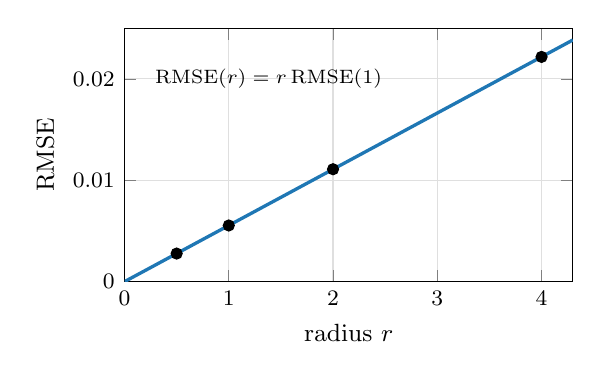
\begin{tikzpicture}
\begin{axis}[width=0.6\textwidth, height=4.8cm, xmin=0, xmax=4.3, ymin=0, ymax=0.025,
  xlabel={radius $r$}, ylabel={RMSE}, scaled y ticks=false,
  yticklabel style={/pgf/number format/fixed, /pgf/number format/precision=3}]
  \addplot[cA, very thick, domain=0:4.3, samples=2] {0.005544*x};
  \addplot[only marks, mark=*, black] coordinates {(0.5,0.00277) (1,0.00554) (2,0.01109) (4,0.02217)};
  \node[font=\scriptsize, anchor=west] at (axis cs:0.2,0.02) {$\mathrm{RMSE}(r) = r\,\mathrm{RMSE}(1)$};
\end{axis}
\end{tikzpicture}
\end{center}

\ans{Q2}
A large radius multiplies the error on every value you actually use. If the signal only spans $[-1, 1]$, radius $4$ makes the error four times larger for no benefit. Choose the radius to match the expected range.

At $x = 1.5$ with radius $1$: neurons with $e = +1$ keep speeding up toward their ceilings, neurons with $e = -1$ stay silent, and the decoders, which were only fitted on $[-1, 1]$, extrapolate. The decoded value is usually somewhere between $1$ and $1.5$ and its error grows with distance. It is not exactly $1$, because nothing in an LIF population clips hard at the radius.
\begin{result}
$\mathrm{RMSE} \propto r$. A radius smaller than the signal causes extrapolation error; a radius larger than needed wastes precision.
\end{result}

\section{Encoding a 2-D vector}

\ans{Q1}
\[
J_1 = 2(0.6) + 1 = 2.2, \qquad J_2 = 2(0.8) + 1 = 2.6, \qquad J_3 = 2(-0.36 - 0.64) + 1 = -1.
\]
Neurons 1 and 2 fire ($J > 1$); neuron 3 is silent. Among unit inputs, $\langle e_3, x\rangle$ is largest for $x = e_3 = (-0.6, -0.8)$, which gives $J_3 = 3$.

\ans{Q2}
$J = \frac{x_1 + x_2}{\sqrt2} + \frac12 > 1 \iff x_1 + x_2 > \frac{\sqrt2}{2} \approx 0.71$. This is the part of the disc beyond a line perpendicular to $e$, at distance $\frac12$ from the origin along $e$.
\begin{center}
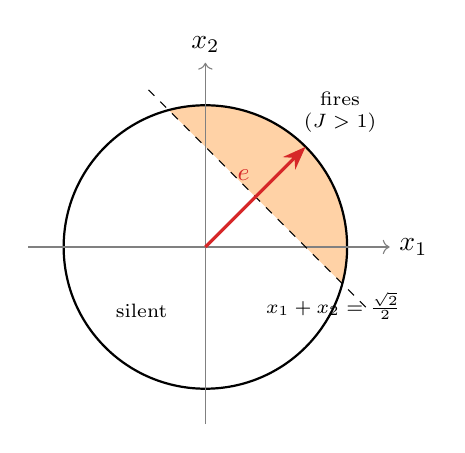
\begin{tikzpicture}[scale=1.8]
  \begin{scope}
    \clip (0,0) circle (1);
    \fill[orange!35, rotate=45] (0.5,-1.5) rectangle (1.5,1.5);
  \end{scope}
  \draw[thick] (0,0) circle (1);
  \draw[->, gray] (-1.25,0) -- (1.3,0) node[right, black] {$x_1$};
  \draw[->, gray] (0,-1.25) -- (0,1.3) node[above, black] {$x_2$};
  \draw[dashed, rotate=45] (0.5,-1.1) -- (0.5,1.1);
  \draw[-{Stealth}, very thick, cD] (0,0) -- (0.707,0.707) node[pos=0.55, above left, font=\small] {$e$};
  \node[font=\scriptsize, align=center] at (0.95,0.95) {fires\\($J>1$)};
  \node[font=\scriptsize] at (-0.45,-0.45) {silent};
  \node[font=\scriptsize, anchor=north west] at (0.36,-0.25) {$x_1 + x_2 = \tfrac{\sqrt2}{2}$};
\end{tikzpicture}
\end{center}
\begin{result}
$J = (2.2, 2.6, -1)$: neurons 1 and 2 fire. The second neuron fires for $x_1 + x_2 > \sqrt2/2$, a cap of the disc on the encoder side.
\end{result}

\section{Decoding a 2-D vector, with shapes}

\ans{Q1}
\begin{center}
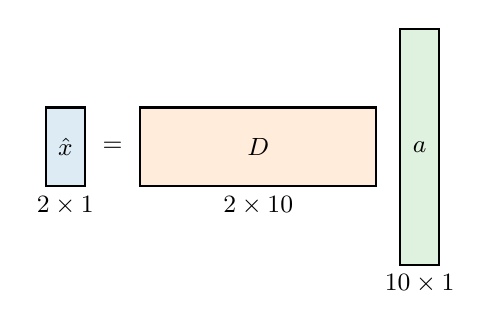
\begin{tikzpicture}[font=\small]
  \draw[thick, fill=cA!15] (0,0) rectangle (0.5,1.0); \node at (0.25,0.5) {$\hat x$}; \node[below] at (0.25,0) {$2\times1$};
  \node at (0.85,0.5) {$=$};
  \draw[thick, fill=cB!15] (1.2,0) rectangle (4.2,1.0); \node at (2.7,0.5) {$D$}; \node[below] at (2.7,0) {$2\times10$};
  \draw[thick, fill=cC!15] (4.5,-1.0) rectangle (5.0,2.0); \node at (4.75,0.5) {$a$}; \node[below] at (4.75,-1.0) {$10\times1$};
\end{tikzpicture}
\end{center}
\[
D^\T = (AA^\T + N\sigma^2 I_{10})^{-1}AX^\T,
\]
with $A$ of shape $10 \times N$, $X$ of shape $2 \times N$, $AA^\T$ and $I_{10}$ of shape $10 \times 10$, $AX^\T$ of shape $10 \times 2$, and $D^\T$ of shape $10 \times 2$.

\ans{Q2}
$f(x) = x_1x_2$ is one number, so its decoder is $1 \times 10$. It needs its own least-squares fit with targets $x_1x_2$. The swap $(x_2, x_1) = Px$ with $P = \begin{pmatrix}0 & 1\\1 & 0\end{pmatrix}$ is linear, so its decoder is $PD$: the two rows of $D$ swapped, $2 \times 10$. Linear functions of $x$ reuse the identity decoder; nonlinear functions need a new solve.
\begin{result}
$\hat x = Da$: $(2\times10)(10\times1)$. \ $D^{x_1x_2}$ is $1\times10$. \ $D^{(x_2,x_1)} = PD$.
\end{result}

\section{Linear transformations of vectors}

\ans{Q1}
\[
v = 2(0.3, -0.2) - (0.4, 0.1) + 3(-0.1, 0.2) = (0.6 - 0.4 - 0.3,\ -0.4 - 0.1 + 0.6) = (-0.1,\ 0.1),
\]
so $\|v\| = \sqrt{0.02} \approx 0.14$.
Connections into $v$: from $a$ with \texttt{transform=2}, from $b$ with \texttt{transform=-1}, from $c$ with \texttt{transform=3}. Each scalar means that multiple of $I_2$.

\ans{Q2}
$v_1(t) = 0.6 - 0.9\sin 2\pi t - 0.3 = 0.3 - 0.9\sin 2\pi t \in [-0.6,\ 1.2]$, and $v_2 = 0.1$. The largest norm is $\sqrt{1.2^2 + 0.1^2} = \sqrt{1.45} \approx 1.20$. $\|v\| > 1$ when $v_1 > \sqrt{0.99} \approx 0.995$, that is $\sin 2\pi t < -0.772$, so $t \in (0.64,\ 0.86)$ s in each second.

PN3 \S1b: $w_1 = 0.5 - 3\sin 4\pi t + 0.4 - 2\sin 4\pi t = 0.9 - 5\sin 4\pi t \in [-4.1,\ 5.9]$, with $w_2 = 0.7$. That is far outside radius $1$. The decoded $w$ will be badly wrong for most of the cycle unless $w$ gets a radius near $6$.
\begin{center}
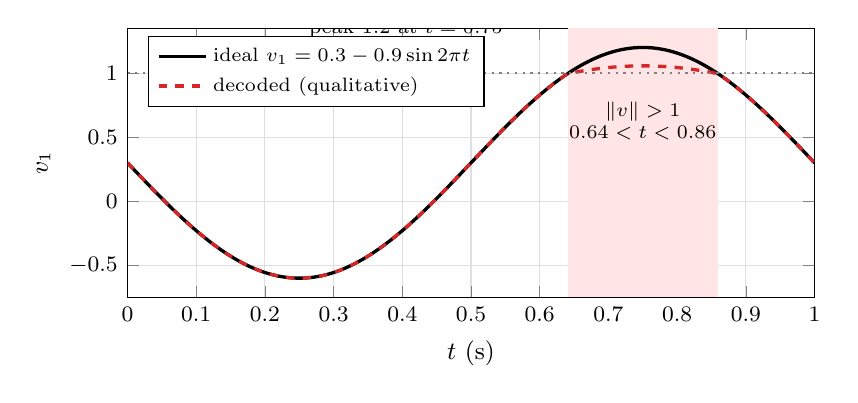
\begin{tikzpicture}
\begin{axis}[width=0.85\textwidth, height=5cm, xmin=0, xmax=1, ymin=-0.75, ymax=1.35,
  xlabel={$t$ (s)}, ylabel={$v_1$}, legend pos=north west, legend cell align=left]
  \fill[red!10] (axis cs:0.641,-0.75) rectangle (axis cs:0.859,1.35);
  \addplot[black, very thick, domain=0:1, samples=200] {0.3 - 0.9*sin(deg(2*pi*x))};
  \addplot[cD, very thick, dashed, domain=0:1, samples=300] {min(0.3 - 0.9*sin(deg(2*pi*x)), 0.995 + 0.3*(0.3 - 0.9*sin(deg(2*pi*x)) - 0.995))};
  \addplot[gray, dotted, thick, domain=0:1, samples=2] {1};
  \legend{ideal $v_1 = 0.3 - 0.9\sin 2\pi t$, decoded (qualitative)}
  \node[font=\scriptsize, anchor=north, align=center] at (axis cs:0.75,0.85) {$\|v\| > 1$\\$0.64 < t < 0.86$};
  \node[font=\scriptsize, anchor=south west] at (axis cs:0.25,1.2) {peak $1.2$ at $t = 0.75$};
\end{axis}
\end{tikzpicture}
\end{center}
\begin{result}
$v = (-0.1, 0.1)$, $\|v\| \approx 0.14$. With the sine: $v_1 \in [-0.6, 1.2]$, $\max\|v\| \approx 1.2$, outside the radius for $0.64 < t < 0.86$ s. PN3's $w_1 \in [-4.1, 5.9]$.
\end{result}

\section{Synapses in a chain, and probe filters}

\ans{Q1}
One synapse: $x(t) = 1 - e^{-t/\tau}$, so $x(\tau) = 1 - e^{-1} \approx 0.63$ and $x(3\tau) = 1 - e^{-3} \approx 0.95$.
Two synapses: $x(t) = 1 - (1 + t/\tau)e^{-t/\tau}$, so $x(\tau) = 1 - 2e^{-1} \approx 0.26$ and $x(3\tau) = 1 - 4e^{-3} \approx 0.80$. The second filter makes the start flat (zero slope at $t = 0$) and adds lag.

\ans{Q2}
Input to A's probe: the input connection plus the probe, so $2$ synapses. Input to B's probe: input connection, A$\to$B, and the probe, so $3$. B's trace is the most rounded and the most delayed.

For $y = 1 - 2x$, the constant $1$ is decoded from A all the time, so B's probe climbs from $0$ to $1$ at the start of the run (two synapses: A$\to$B and the probe). During the pulse it heads to $1 - 2 = -1$ with the three-synapse lag, and it returns to $1$ after $0.4$ s.
\begin{center}
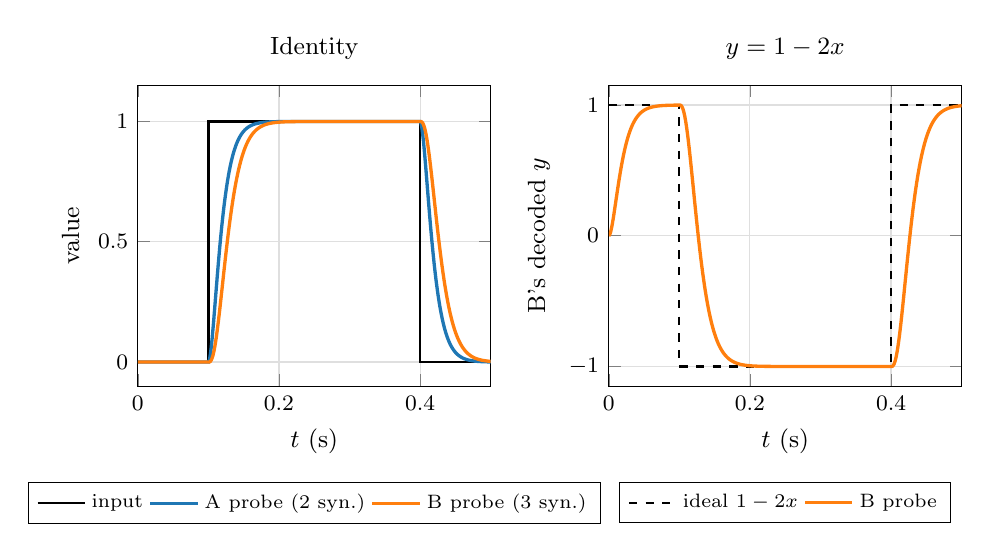
\begin{tikzpicture}[
  declare function={
    Sone(\t) = 1 - exp(-max(\t,0)/0.01);
    Stwo(\t) = 1 - exp(-max(\t,0)/0.01)*(1 + max(\t,0)/0.01);
    Sthree(\t) = 1 - exp(-max(\t,0)/0.01)*(1 + max(\t,0)/0.01 + (max(\t,0)/0.01)^2/2);}]
\begin{groupplot}[group style={group size=2 by 1, horizontal sep=1.5cm},
  width=0.5\textwidth, height=5.4cm, xmin=0, xmax=0.5, xlabel={$t$ (s)},
  legend cell align=left, legend style={at={(0.5,-0.32)}, anchor=north, legend columns=3}]
\nextgroupplot[ylabel={value}, ymin=-0.1, ymax=1.15, title={Identity}]
  \addplot[black, thick] coordinates {(0,0) (0.1,0) (0.1,1) (0.4,1) (0.4,0) (0.5,0)};
  \addplot[cA, very thick, domain=0:0.5, samples=400] {Stwo(x-0.1) - Stwo(x-0.4)};
  \addplot[cB, very thick, domain=0:0.5, samples=400] {Sthree(x-0.1) - Sthree(x-0.4)};
  \legend{input, A probe (2 syn.), B probe (3 syn.)}
\nextgroupplot[ylabel={B's decoded $y$}, ymin=-1.15, ymax=1.15, title={$y = 1 - 2x$}]
  \addplot[black, thick, dashed] coordinates {(0,1) (0.1,1) (0.1,-1) (0.4,-1) (0.4,1) (0.5,1)};
  \addplot[cB, very thick, domain=0:0.5, samples=400] {Stwo(x) - 2*(Sthree(x-0.1) - Sthree(x-0.4))};
  \legend{ideal $1 - 2x$, B probe}
\end{groupplot}
\end{tikzpicture}
\end{center}
\begin{result}
One synapse: $0.63$ at $\tau$, $0.95$ at $3\tau$. Two: $0.26$, $0.80$. A's probe sits behind $2$ synapses and B's behind $3$. For $1 - 2x$, B starts by rising to $1$, dips to $-1$ during the pulse, and returns to $1$.
\end{result}

\section{Nengo vocabulary}

\ans{Q1}
\begin{lstlisting}[language=Python]
model = nengo.Network(seed=556)
with model:
    stim = nengo.Node(lambda t: 1.0 if 0.1 < t < 0.4 else 0.0)
    params = dict(intercepts=nengo.dists.Uniform(-1, 1),
                  max_rates=nengo.dists.Uniform(100, 200))
    a = nengo.Ensemble(100, dimensions=1, **params)
    b = nengo.Ensemble(50, dimensions=1, **params)
    nengo.Connection(stim, a)
    nengo.Connection(a, b, function=lambda x: 1 - 2 * x, synapse=0.01)
    p_in = nengo.Probe(stim)
    p_a = nengo.Probe(a, synapse=0.01)
    p_b = nengo.Probe(b, synapse=0.01)
with nengo.Simulator(model) as sim:
    sim.run(0.5)
\end{lstlisting}
\texttt{transform=-2} alone would give $-2x$. The offset $+1$ is not linear in $x$, so it needs \texttt{function=}.

\ans{Q2}
\begin{enumerate}[label=(\arabic*)]
\item Line 5, input \texttt{transform=1}: it should be $B' = \tau B = \tau$, so \texttt{transform=tau}. With $1$ the integral is $1/\tau = 20$ times too fast.
\item Line 6, recurrent \texttt{transform=tau}: it should be $A' = \tau\cdot 0 + 1 = 1$. With $\tau$ the feedback is $0.05x$, a strong leak rather than memory.
\item Line 6, recurrent \texttt{synapse=0.005}: $A'$ and $B'$ were derived for the recurrent synapse, so it must be \texttt{synapse=tau} ($50$ ms).
\end{enumerate}
\begin{result}
Input: \texttt{transform=tau, synapse=0.005}. Recurrent: \texttt{transform=1, synapse=tau}.
\end{result}

%=====================================================================
\part*{Part B}
%=====================================================================

\section{Two Laplace facts}

\ans{Q1}
\[
H(s) = \int_0^\infty \frac1\tau e^{-t/\tau}e^{-st}\,dt = \frac1\tau\int_0^\infty e^{-t(s + 1/\tau)}dt
= \frac1\tau\left[\frac{-e^{-t(s + 1/\tau)}}{s + 1/\tau}\right]_0^\infty = \frac1\tau\cdot\frac{1}{s + 1/\tau} = \frac{1}{1 + s\tau}.
\]
The upper limit is $0$ because $\mathrm{Re}(s) > -1/\tau$; the lower limit gives $-1/(s + 1/\tau)$, and the minus signs cancel.

\ans{Q2}
With $a = s + 1/\tau$, integration by parts gives $\int_0^\infty t e^{-at}dt = \bigl[-\tfrac{t}{a}e^{-at}\bigr]_0^\infty + \tfrac1a\int_0^\infty e^{-at}dt = \tfrac{1}{a^2}$. So
\[
\mathcal{L}\{h_1\} = \frac{1}{\tau^2(s + 1/\tau)^2} = \frac{1}{(1 + s\tau)^2} = H(s)^2.
\]
$h_1$ is two exponential synapses in series, which is why its step response matched the two-synapse curve in Section~6.

Derivative check: $x = e^{-at}$ has $X = 1/(s + a)$. Directly, $\mathcal{L}\{-ae^{-at}\} = -a/(s + a)$. The rule gives $sX - x(0) = \frac{s}{s + a} - 1 = \frac{-a}{s + a}$. They agree. Lecture~6 drops $x(0)$ because the signals start at zero.
\begin{result}
$H(s) = 1/(1 + s\tau)$. \ $\mathcal{L}\{h_1\} = 1/(1 + s\tau)^2$. \ $\mathcal{L}\{\dot x\} = sX - x(0)$.
\end{result}

\section{The recurrent connection is a differential equation}

\ans{Q1}
\begin{align*}
x &= h * (g(u) + f(x)) && \text{the population represents its filtered total input}\\
X(s) &= \frac{1}{1 + s\tau}\bigl(G(s) + F(s)\bigr) && \text{convolution becomes multiplication by } H(s)\\
X(1 + s\tau) &= G + F && \text{multiply through}\\
s\tau X &= G + F - X && \text{isolate the } s \text{ term}\\
\tau\dot x &= g(u) + f(x) - x && s \text{ becomes } d/dt
\end{align*}

\ans{Q2}
$y(t) = \int_{-\infty}^t \frac1\tau e^{-(t - t')/\tau}z(t')\,dt'$. Differentiating the upper limit gives $\frac1\tau z(t)$, and differentiating the integrand gives $-\frac1\tau y(t)$. So $\dot y = (z - y)/\tau$, which is $\tau\dot y = z - y$. Substituting $z = g(u) + f(x)$ and $y = x$ gives the same equation.

The synapse integrates its input (the $z/\tau$ term) but loses its own value at rate $y/\tau$ (the leak). Left alone it forgets with time constant $\tau$. That is a leaky integrator.
\begin{result}
$\tau\dot x = g(u) + f(x) - x$. The $-x$ is the synaptic leak.
\end{result}

\section{Linear feedback $f(x) = kx$}

\ans{Q1}
$\tau\dot x = u - 2x$, so $\dot x = \frac{2}{\tau}\bigl(\tfrac{u}{2} - x\bigr)$ and $x(t) = \tfrac12\bigl(1 - e^{-2t/\tau}\bigr)$. The steady state is $\tfrac12$ and the time constant is $\tau/2 = 25$ ms. The lecture's ``converges to $u/2$'' is the steady state. The equation also says the loop approaches it twice as fast as the synapse alone.

\ans{Q2}
\begin{itemize}[leftmargin=1.2em]
\item $k = 0.5$: $\tau\dot x = u - 0.5x$, so $x = 2(1 - e^{-t/(2\tau)})$. The steady state $2$ is outside radius $1$, so the neural trace bends over near $1$. Time constant $2\tau = 100$ ms.
\item $k = 1$: $\tau\dot x = u$, so $x = t/\tau = 20t$, which reaches the radius at $t = 50$ ms. An integrator.
\item $k = 2$: $\tau\dot x = u + x$, so $x = e^{t/\tau} - 1$, which reaches $1$ at $t = \tau\ln 2 \approx 35$ ms. Unstable.
\end{itemize}
Lecture's $f(x) = x + 1$: $\tau\dot x = u + x + 1 - x = u + 1$. The $x$ terms cancel, so it is an integrator of $u + 1$. With $u = 0$ it ramps at $1/\tau$ forever. The ``convergence slightly above $1$'' in the lecture is saturation, not a real equilibrium.
\begin{center}
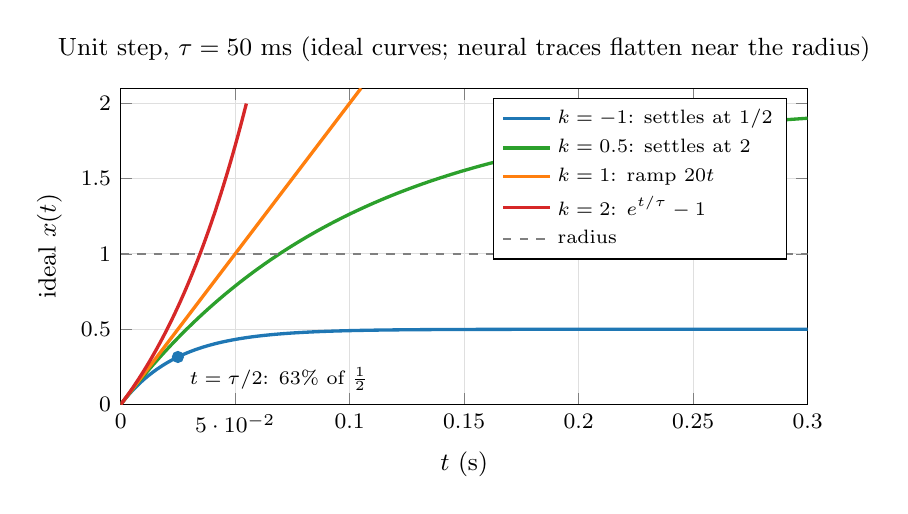
\begin{tikzpicture}
\begin{axis}[width=0.85\textwidth, height=5.6cm, xmin=0, xmax=0.3, ymin=0, ymax=2.1,
  xlabel={$t$ (s)}, ylabel={ideal $x(t)$}, legend pos=north east, legend cell align=left,
  title={Unit step, $\tau = 50$ ms (ideal curves; neural traces flatten near the radius)}]
  \addplot[cA, very thick, domain=0:0.3, samples=150] {0.5*(1-exp(-2*x/0.05))};
  \addplot[cC, very thick, domain=0:0.3, samples=150] {2*(1-exp(-x/0.1))};
  \addplot[cB, very thick, domain=0:0.105, samples=50] {20*x};
  \addplot[cD, very thick, domain=0:0.0549, samples=80] {exp(x/0.05)-1};
  \addplot[gray, dashed, thick, domain=0:0.3, samples=2] {1};
  \legend{{$k=-1$: settles at $1/2$}, {$k=0.5$: settles at $2$}, {$k=1$: ramp $20t$}, {$k=2$: $e^{t/\tau}-1$}, radius}
  \addplot[only marks, mark=*, cA, forget plot] coordinates {(0.025,0.316)};
  \node[font=\scriptsize, anchor=north west] at (axis cs:0.026,0.31) {$t = \tau/2$: $63\%$ of $\frac12$};
\end{axis}
\end{tikzpicture}
\end{center}
\begin{result}
$k = -1$: $\frac12(1 - e^{-2t/\tau})$. \ $k = 0.5$: $2(1 - e^{-t/2\tau})$. \ $k = 1$: $t/\tau$. \ $k = 2$: $e^{t/\tau} - 1$. \ $f = x + 1$ is an integrator of $u + 1$.
\end{result}

\section{One-dimensional phase portraits and stability}

\ans{Q1}
$\tau\phi = u + x^2 - x$. At $u = 0.16$: $x^2 - x + 0.16 = 0$, so $x = \frac{1 \pm \sqrt{1 - 0.64}}{2} = \frac{1 \pm 0.6}{2} = 0.2$ or $0.8$. With $\tau\phi' = 2x - 1$: at $0.2$ it is $-0.6$ (stable), and at $0.8$ it is $+0.6$ (unstable).

At $u = 0.3$ the discriminant $1 - 1.2$ is negative, so there is no equilibrium and $\phi > 0$ everywhere: $x$ grows until it saturates. Ideally the jump happens at $u = 1/4$. The lecture saw about $0.4$ because the neural version is distorted and saturates.

With $x(0) = 1$ and $u = 0.16$ the state starts right of the unstable point, so it runs away upward and never returns to $0.2$. The same input gives different outcomes depending on where the state was. That history dependence is the lecture's ``memory''.

\ans{Q2}
(i) $\tau\phi = -x^3$. The only equilibrium is $x = 0$. Here $\phi'(0) = 0$, but the arrows point inward on both sides, so it is stable. Convergence is slow and not exponential.

(ii) $\tau\phi = x(0.25 - x^2)$, with zeros at $0$ and $\pm 0.5$. $\tau\phi' = 0.25 - 3x^2$: $+0.25$ at $0$ (unstable), $-0.5$ at $\pm0.5$ (stable). (ii) stores one bit, the sign of $x$: any start with $x > 0$ settles at $+0.5$, and any start with $x < 0$ settles at $-0.5$.
\begin{center}
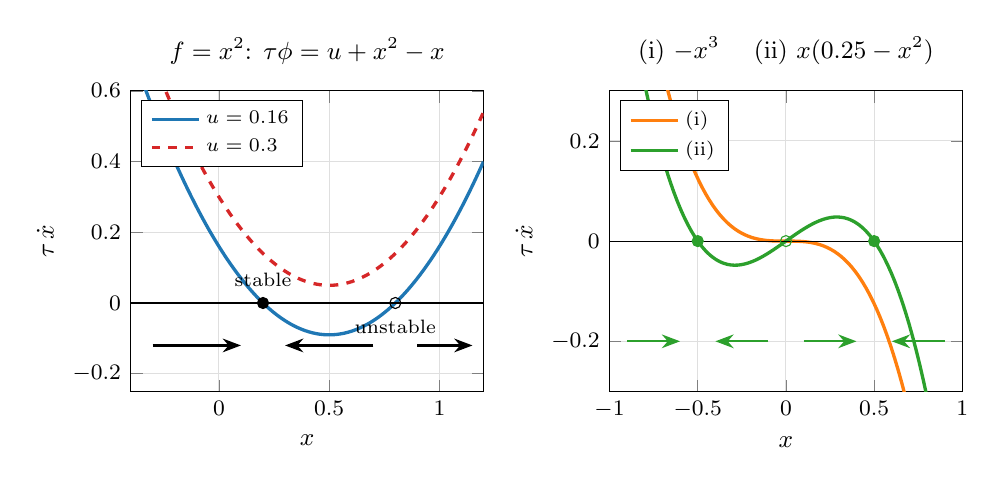
\begin{tikzpicture}
\begin{groupplot}[group style={group size=2 by 1, horizontal sep=1.6cm},
  width=0.5\textwidth, height=5.4cm, legend pos=north west, legend cell align=left]
\nextgroupplot[xmin=-0.4, xmax=1.2, ymin=-0.25, ymax=0.6, xlabel={$x$}, ylabel={$\tau\,\dot x$},
  title={$f = x^2$: $\tau\phi = u + x^2 - x$}]
  \addplot[cA, very thick, domain=-0.4:1.2, samples=100] {0.16 + x^2 - x};
  \addplot[cD, very thick, dashed, domain=-0.4:1.2, samples=100] {0.3 + x^2 - x};
  \addplot[black, domain=-0.4:1.2, samples=2] {0};
  \legend{$u = 0.16$, $u = 0.3$}
  \addplot[only marks, mark=*, black] coordinates {(0.2,0)};
  \addplot[only marks, mark=o, black, mark options={fill=white}] coordinates {(0.8,0)};
  \draw[-{Stealth}, thick] (axis cs:-0.3,-0.12) -- (axis cs:0.1,-0.12);
  \draw[-{Stealth}, thick] (axis cs:0.7,-0.12) -- (axis cs:0.3,-0.12);
  \draw[-{Stealth}, thick] (axis cs:0.9,-0.12) -- (axis cs:1.15,-0.12);
  \node[font=\scriptsize, anchor=south] at (axis cs:0.2,0.02) {stable};
  \node[font=\scriptsize, anchor=north] at (axis cs:0.8,-0.02) {unstable};
\nextgroupplot[xmin=-1, xmax=1, ymin=-0.3, ymax=0.3, xlabel={$x$}, ylabel={$\tau\,\dot x$},
  title={(i) $-x^3$ \quad (ii) $x(0.25 - x^2)$}]
  \addplot[cB, very thick, domain=-1:1, samples=100] {-x^3};
  \addplot[cC, very thick, domain=-1:1, samples=100] {x*(0.25-x^2)};
  \addplot[black, domain=-1:1, samples=2] {0};
  \legend{(i), (ii)}
  \addplot[only marks, mark=*, cC] coordinates {(-0.5,0) (0.5,0)};
  \addplot[only marks, mark=o, cC, mark options={fill=white}] coordinates {(0,0)};
  \draw[-{Stealth}, thick, cC] (axis cs:0.1,-0.2) -- (axis cs:0.4,-0.2);
  \draw[-{Stealth}, thick, cC] (axis cs:0.9,-0.2) -- (axis cs:0.6,-0.2);
  \draw[-{Stealth}, thick, cC] (axis cs:-0.1,-0.2) -- (axis cs:-0.4,-0.2);
  \draw[-{Stealth}, thick, cC] (axis cs:-0.9,-0.2) -- (axis cs:-0.6,-0.2);
\end{groupplot}
\end{tikzpicture}
\end{center}
Filled dots are stable and open dots unstable. Arrows show the direction of motion along $x$.
\begin{result}
$u = 0.16$: stable $0.2$, unstable $0.8$; no equilibrium for $u > 1/4$. \ (i) one slow stable point at $0$. \ (ii) stable $\pm0.5$, unstable $0$; it stores the sign of $x$.
\end{result}

\section{Mapping an LTI system onto a synapse}

\ans{Q1}
$X = \frac{1}{1 + s\tau}(A'X + B'U) \Rightarrow s\tau X = (A' - I)X + B'U \Rightarrow sX = \frac{A' - I}{\tau}X + \frac{B'}{\tau}U$. Matching with $sX = AX + BU$ gives $A = (A' - I)/\tau$ and $B = B'/\tau$, so $A' = \tau A + I$ and $B' = \tau B$.

Integrator: $A = 0$, $B = I_d$, so $A' = I_d$ and $B' = 0.05\,I_d$.

\ans{Q2}
$A = -1/\tau_d$, $B = 1/\tau_d$.
\[
\tau_d = 200\ \mathrm{ms}: \ A' = 1 - \tfrac{0.05}{0.2} = 0.75,\ B' = 0.25. \qquad
\tau_d = 10\ \mathrm{ms}: \ A' = 1 - \tfrac{0.05}{0.01} = -4,\ B' = 5.
\]
Steady state $x = A'x + B'u$: $0.25x = 0.25u$ and $5x = 5u$, so both give $x = u$.

The surprise: with $\tau_d = 10$ ms the network responds five times faster than its own $50$ ms synapses. Strong negative feedback ($A' = -4$) combined with a large input gain speeds the loop up. The network-level time constant is a design choice, separate from the synapse's.
\begin{center}
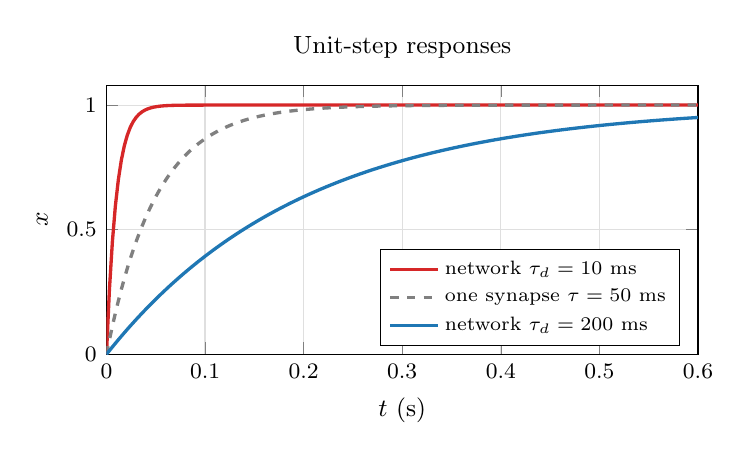
\begin{tikzpicture}
\begin{axis}[width=0.75\textwidth, height=5cm, xmin=0, xmax=0.6, ymin=0, ymax=1.08,
  xlabel={$t$ (s)}, ylabel={$x$}, legend pos=south east, legend cell align=left,
  title={Unit-step responses}, scaled x ticks=false, xticklabel style={/pgf/number format/fixed}]
  \addplot[cD, very thick, domain=0:0.6, samples=200] {1-exp(-x/0.01)};
  \addplot[gray, very thick, dashed, domain=0:0.6, samples=200] {1-exp(-x/0.05)};
  \addplot[cA, very thick, domain=0:0.6, samples=200] {1-exp(-x/0.2)};
  \legend{network $\tau_d = 10$ ms, one synapse $\tau = 50$ ms, network $\tau_d = 200$ ms}
\end{axis}
\end{tikzpicture}
\end{center}
\begin{result}
$A' = \tau A + I$, $B' = \tau B$. Integrator: $A' = I$, $B' = 0.05I$. Low-pass: $(0.75, 0.25)$ for $200$ ms, $(-4, 5)$ for $10$ ms.
\end{result}

\section{The ideal answer is a definite integral}

\ans{Q1}
\[
x(t) = \int_0^t u = \begin{cases} 0, & t < 0.2,\\ 0.8(t - 0.2), & 0.2 \le t < 1.0,\\ 0.64, & t \ge 1.0. \end{cases}
\]
\begin{center}
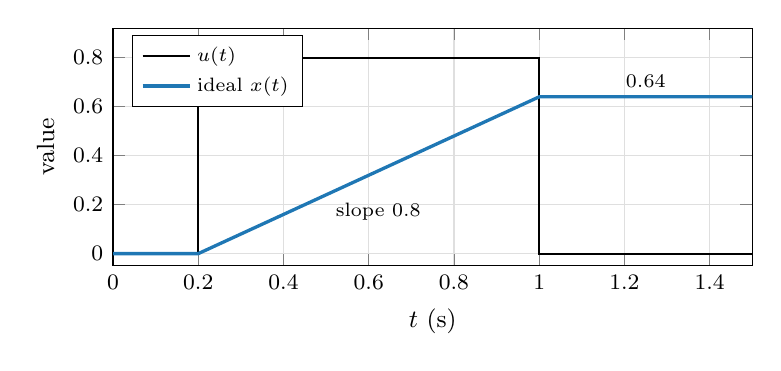
\begin{tikzpicture}
\begin{axis}[width=0.8\textwidth, height=4.6cm, xmin=0, xmax=1.5, ymin=-0.05, ymax=0.92,
  xlabel={$t$ (s)}, ylabel={value}, legend pos=north west, legend cell align=left]
  \addplot[black, thick] coordinates {(0,0) (0.2,0) (0.2,0.8) (1.0,0.8) (1.0,0) (1.5,0)};
  \addplot[cA, very thick] coordinates {(0,0) (0.2,0) (1.0,0.64) (1.5,0.64)};
  \legend{$u(t)$, ideal $x(t)$}
  \node[font=\scriptsize, anchor=south] at (axis cs:1.25,0.64) {$0.64$};
  \node[font=\scriptsize, anchor=west] at (axis cs:0.5,0.17) {slope $0.8$};
\end{axis}
\end{tikzpicture}
\end{center}

\ans{Q2}
(i) The ramp is $u = 2t$ on $[0, 0.3)$, so $x = t^2$ there and then holds at $0.09$.

(ii) $x = \int_0^t 3\sin 3t'\,dt' = \bigl[-\cos 3t'\bigr]_0^t = 1 - \cos 3t$. Its range is $[0, 2]$, which exceeds radius $1$.

The neural state saturates near $1$ at $t = \pi/6 \approx 0.52$ s, while the ideal keeps climbing to $2$ at $t = \pi/3$. The integrator only stores its current value, so when $u$ goes negative it comes down by the full integral and ends up $1$ below the ideal. From then on it traces $1 - \cos 3t - 1 = -\cos 3t$, which fits inside the radius. The simulated $400$-neuron trace does exactly this. PN3's $5\sin 5t$ (ideal $1 - \cos 5t$) has the same problem.
\begin{center}
\begin{tikzpicture}
\begin{groupplot}[group style={group size=2 by 1, horizontal sep=1.5cm},
  xlabel={$t$ (s)}, legend cell align=left]
\nextgroupplot[width=0.38\textwidth, height=5cm, xmin=0, xmax=0.5, ymin=-0.02, ymax=0.65, title={(i) ramp}, legend pos=north west]
  \addplot[black, thick] coordinates {(0,0) (0.3,0.6) (0.3,0) (0.5,0)};
  \addplot[cA, very thick, domain=0:0.3, samples=60] {x^2};
  \addplot[cA, very thick, forget plot] coordinates {(0.3,0.09) (0.5,0.09)};
  \legend{$u = 2t$, $x = t^2$}
  \node[font=\scriptsize, anchor=south] at (axis cs:0.42,0.09) {$0.09$};
\nextgroupplot[width=0.6\textwidth, height=5cm, xmin=0, xmax=4, ymin=-1.2, ymax=2.15, title={(ii) $u = 3\sin 3t$, radius $1$}, legend style={at={(0.5,0.02)}, anchor=south, legend columns=3}]
  \addplot[black, very thick, domain=0:4, samples=200] {1-cos(deg(3*x))};
  \addplot[cD, very thick] table[x=t, y=x] {pn3_data/sine_saturation.dat};
  \addplot[cC, thick, dashed, domain=1.047:4, samples=150] {-cos(deg(3*x))};
  \addplot[gray, dotted, thick, domain=0:4, samples=2, forget plot] {1};
  \legend{ideal $1 - \cos 3t$, Nengo (400 rate neurons), $-\cos 3t$}
\end{groupplot}
\end{tikzpicture}
\end{center}
\begin{result}
Step: $0$, \ $0.8(t - 0.2)$, \ $0.64$. \ Ramp: $t^2$, then $0.09$. \ Sine: $1 - \cos 3t \in [0, 2]$; the neural trace clips once, then follows about $-\cos 3t$.
\end{result}

\section{Why a neural integrator drifts}

\ans{Q1}
Read the sign of $\hat\phi$ at the start, then follow it to the next zero where $\hat\phi$ crosses downward.
\begin{itemize}[leftmargin=1.2em]
\item $x = 0.3$: $\hat\phi \approx +0.1\ \mathrm{s^{-1}}$, so it moves up to the stable zero near $0.37$. It covers $0.07$ at under $0.15$ per second, slowing as it arrives: on the order of a second.
\item $x = -0.3$: $\hat\phi \approx +0.27$, so it moves up to the stable zero near $0$. This takes one to two seconds.
\item $x = 0.6$: $\hat\phi \approx +0.36$, so it moves up to the stable zero near $0.76$, in well under a second.
\end{itemize}
The stable zeros (downward crossings) are near $-0.90, -0.75, 0, 0.16, 0.37, 0.76$. The unstable ones are near $-0.82, -0.48, 0.01, 0.23, 0.51$.
\begin{center}
\begin{tikzpicture}
\begin{axis}[width=0.9\textwidth, height=5.4cm, xmin=-1, xmax=1, ymin=-0.85, ymax=0.85,
  xlabel={represented value $x$}, ylabel={$\hat\phi(x)$ (s$^{-1}$)}, xtick={-1,-0.8,...,1}]
  \addplot[black, thick, domain=-1:1, samples=2] {0};
  \addplot[blue!70!black, very thick] table[x=x, y=phi] {pn3_data/neural_phase.dat};
  \addplot[only marks, mark=*, black] coordinates {(-0.898,0) (-0.748,0) (-0.005,0) (0.159,0) (0.371,0) (0.756,0)};
  \addplot[only marks, mark=o, black, mark options={fill=white}] coordinates {(-0.821,0) (-0.477,0) (0.013,0) (0.231,0) (0.509,0)};
  \draw[-{Stealth}, very thick, cD] (axis cs:0.3,-0.5) -- (axis cs:0.37,-0.5);
  \draw[-{Stealth}, very thick, cD] (axis cs:-0.3,-0.5) -- (axis cs:-0.02,-0.5);
  \draw[-{Stealth}, very thick, cD] (axis cs:0.6,-0.5) -- (axis cs:0.75,-0.5);
  \node[font=\scriptsize, cD] at (axis cs:-0.15,-0.62) {from $-0.3$};
  \node[font=\scriptsize, cD] at (axis cs:0.33,-0.62) {$0.3$};
  \node[font=\scriptsize, cD] at (axis cs:0.67,-0.62) {$0.6$};
\end{axis}
\end{tikzpicture}
\end{center}

\ans{Q2}
In spiking mode, each run adds a different realisation of spike noise to the recurrent input. The state takes a random walk on top of the deterministic drift, so it can be knocked across an unstable zero into a different basin, and repeated runs end in different places. In rate mode there is no spike noise, the dynamics are exactly $\hat\phi$, and the same seed gives the same neurons, so the run repeats.

Doubling the neurons roughly halves the distortion error. The bumps in $\hat\phi$ get smaller (slower drift) and usually more numerous and closer together. The curve never becomes exactly zero.
\begin{result}
Drift to the next stable zero: $0.3 \to 0.37$, \ $-0.3 \to 0$, \ $0.6 \to 0.76$. Static distortion causes deterministic drift; spike noise causes run-to-run variation.
\end{result}

\section{Unequal input and recurrent synapses}

\ans{Q1}
With $A' = 1$ and $B' = \tau$:
\[
X = \frac{X}{1 + s\tau} + \frac{\tau U}{1 + s\tin}
\ \Rightarrow\ X\,\frac{s\tau}{1 + s\tau} = \frac{\tau U}{1 + s\tin}
\ \Rightarrow\ X = \frac{1 + s\tau}{1 + s\tin}\cdot\frac{U}{s}
= \frac{U}{s} + \frac{(\tau - \tin)}{1 + s\tin}\,U.
\]
The first term is the ideal integral. The second is the input itself, filtered by the short synapse and weighted by $\tau - \tin$.

\ans{Q2}
Offset while on: $(\tau - \tin)u = 0.045 \times 0.9 = 0.0405$. The trace jumps up by about $0.04$ within a few ms of $t = 0.04$, then rises parallel to the ideal. At $t = 1.0$ it drops by $0.04$ onto the ideal final value $0.9 \times 0.96 = 0.864$. The end value is unaffected.

If $B'$ were computed with $\tin$, the input gain would be $0.005$ instead of $0.05$, so the network would integrate at one tenth of the rate (final value about $0.086$).
\begin{center}
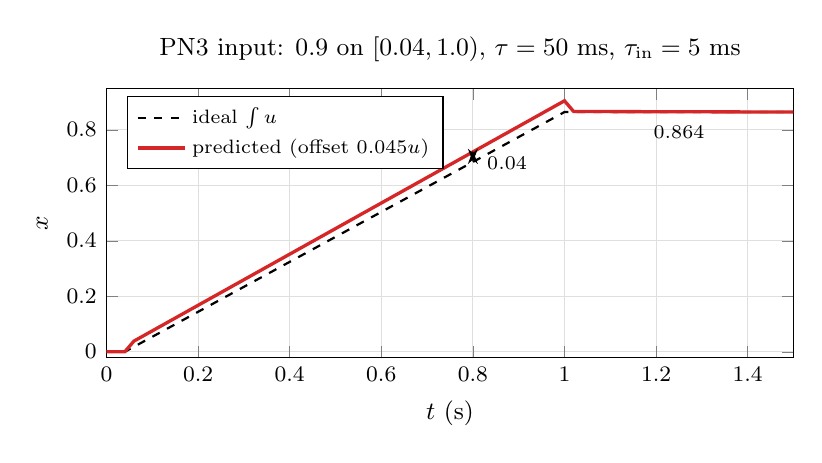
\begin{tikzpicture}
\begin{axis}[width=0.85\textwidth, height=5cm, xmin=0, xmax=1.5, ymin=-0.02, ymax=0.95,
  xlabel={$t$ (s)}, ylabel={$x$}, legend pos=north west, legend cell align=left,
  title={PN3 input: $0.9$ on $[0.04, 1.0)$, $\tau = 50$ ms, $\tin = 5$ ms}]
  \addplot[black, thick, dashed] coordinates {(0,0) (0.04,0) (1.0,0.864) (1.5,0.864)};
  \addplot[cD, very thick] coordinates {(0,0) (0.04,0) (0.06,0.0385) (1.0,0.9045) (1.02,0.866) (1.5,0.864)};
  \legend{ideal $\int u$, predicted (offset $0.045u$)}
  \draw[{Stealth}-{Stealth}] (axis cs:0.8,0.684) -- (axis cs:0.8,0.7245);
  \node[font=\scriptsize, anchor=west] at (axis cs:0.81,0.68) {$0.04$};
  \node[font=\scriptsize, anchor=north] at (axis cs:1.25,0.85) {$0.864$};
\end{axis}
\end{tikzpicture}
\end{center}
\begin{result}
$x = \int u + (\tau - \tin)(h_{\tin} * u)$. Offset $0.0405$ while the input is on; final value $0.864$ as intended.
\end{result}

\section{A leaky integrator: eye position}

\ans{Q1}
$A' = 1 - 0.1/20 = 0.995$ and $B' = 0.1$. With $v = 0$: $x(t) = 0.5e^{-t/20}$, so $x(20) = 0.5/e \approx 0.18$.

\ans{Q2}
$A = (A' - 1)/\tau = -0.02/0.1 = -0.2\ \mathrm{s^{-1}}$, so $\tau_{\mathrm{eff}} = 5$ s and $x = 0.5e^{-t/5}$: $0.5e^{-2} \approx 0.07$ at $10$ s, against $0.5e^{-0.5} \approx 0.30$ intended.
With $A' = 1.01$: $A = +0.1$, so $x = 0.5e^{t/10}$ grows until it saturates.

A decoding error of $1.5\%$ in the recurrent gain cut the memory from $20$ s to $5$ s, and $1\%$ the other way makes it unstable, because $\tau_{\mathrm{eff}} = \tau/(1 - A')$ divides by a tiny number. Long memories need very accurate recurrent decoders, so many neurons or some correction.
\begin{center}
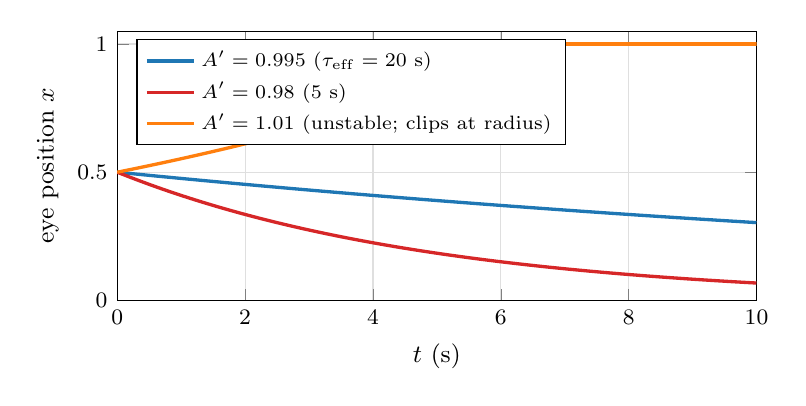
\begin{tikzpicture}
\begin{axis}[width=0.8\textwidth, height=5cm, xmin=0, xmax=10, ymin=0, ymax=1.05,
  xlabel={$t$ (s)}, ylabel={eye position $x$}, legend pos=north west, legend cell align=left]
  \addplot[cA, very thick, domain=0:10, samples=100] {0.5*exp(-x/20)};
  \addplot[cD, very thick, domain=0:10, samples=100] {0.5*exp(-x/5)};
  \addplot[cB, very thick, domain=0:6.93, samples=100] {0.5*exp(x/10)};
  \addplot[cB, very thick, forget plot] coordinates {(6.93,1) (10,1)};
  \legend{$A' = 0.995$ ($\tau_{\mathrm{eff}} = 20$ s), $A' = 0.98$ ($5$ s), $A' = 1.01$ (unstable; clips at radius)}
\end{axis}
\end{tikzpicture}
\end{center}
\begin{result}
$A' = 0.995$, $B' = 0.1$; $x(20) \approx 0.18$. \ $A' = 0.98 \Rightarrow \tau_{\mathrm{eff}} = 5$ s. \ $A' > 1$ is unstable.
\end{result}

\section{The oscillator}

\ans{Q1}
$\omega = 2\pi\cdot 2 = 4\pi$, so $\tau\omega = 0.4\pi \approx 1.26$ and
\[
A' = \begin{pmatrix} 1 & -0.4\pi \\ 0.4\pi & 1 \end{pmatrix}, \qquad B' = 0.
\]
From $(1, 0)$: $x_1 = \cos 4\pi t$ and $x_2 = \sin 4\pi t$. The trajectory is a counter-clockwise circle of radius $1$, once every $0.5$ s.

\ans{Q2}
At $x = 0$, $Ax = 0$, so the origin is an equilibrium and nothing moves without a kick. A huge kick cannot give a huge oscillation, because the neurons saturate at the edge of the represented range. The amplitude settles near the radius, which the lecture describes as a stable cyclic attractor. Noise and distortion can also make a neural oscillator decay to zero.

Damped: $A' = \tau A + I = \begin{pmatrix} 1 - \tau\gamma & -\tau\omega \\ \tau\omega & 1 - \tau\gamma \end{pmatrix}$, with trajectory $e^{-\gamma t}(\cos\omega t, \sin\omega t)$, an inward spiral.
\begin{center}
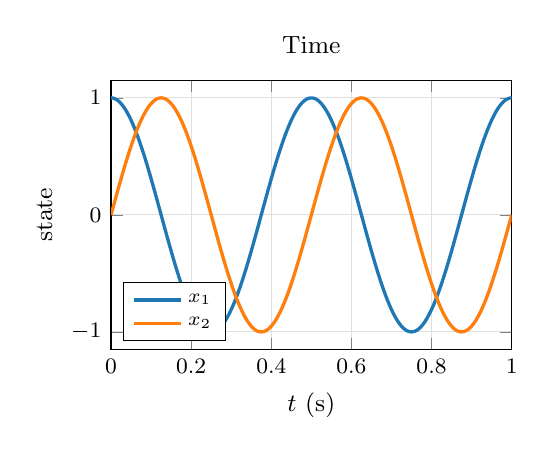
\begin{tikzpicture}
\begin{axis}[width=0.55\textwidth, height=5cm, xmin=0, xmax=1, ymin=-1.15, ymax=1.15,
  xlabel={$t$ (s)}, ylabel={state}, legend pos=south west, legend cell align=left, title={Time}]
  \addplot[cA, very thick, domain=0:1, samples=200] {cos(deg(4*pi*x))};
  \addplot[cB, very thick, domain=0:1, samples=200] {sin(deg(4*pi*x))};
  \legend{$x_1$, $x_2$}
\end{axis}
\end{tikzpicture}\hfill
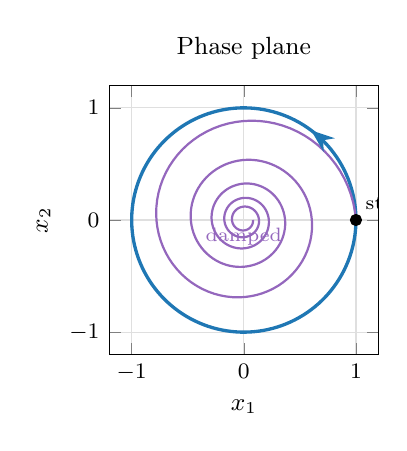
\begin{tikzpicture}
\begin{axis}[width=0.42\textwidth, height=5cm, axis equal image, xmin=-1.2, xmax=1.2, ymin=-1.2, ymax=1.2,
  xlabel={$x_1$}, ylabel={$x_2$}, title={Phase plane}]
  \addplot[cA, very thick, domain=0:0.5, samples=150] ({cos(deg(4*pi*x))},{sin(deg(4*pi*x))});
  \addplot[cE, thick, domain=0:2.5, samples=400] ({exp(-x)*cos(deg(4*pi*x))},{exp(-x)*sin(deg(4*pi*x))});
  \draw[-{Stealth}, very thick, cA] (axis cs:0.71,0.71) -- (axis cs:0.6,0.8);
  \addplot[only marks, mark=*, black] coordinates {(1,0)};
  \node[font=\scriptsize, anchor=west] at (axis cs:1.0,0.15) {start};
  \node[font=\scriptsize, cE] at (axis cs:0,-0.15) {damped};
\end{axis}
\end{tikzpicture}
\end{center}
\begin{result}
$A' = \begin{pmatrix} 1 & -0.4\pi \\ 0.4\pi & 1 \end{pmatrix}$, $B' = 0$. Circle of period $0.5$ s, counter-clockwise; it needs a kick, and its amplitude is set by the radius.
\end{result}

\section{Nonlinear dynamics with the same recipe}

\ans{Q1}
$f'(x) = \tau(-x^3) + x = x - 0.1x^3$ and $g'(u) = 0.1u$.
\begin{lstlisting}[language=Python]
nengo.Connection(stim, x, transform=0.1, synapse=0.1)
nengo.Connection(x, x, function=lambda x: x - 0.1 * x**3, synapse=0.1)
\end{lstlisting}

\ans{Q2}
$f'(x) = \tau\begin{pmatrix} 10x_2 - 10x_1 \\ -x_1x_3 - x_2 \\ x_1x_2 - \tfrac83(x_3 + 28) - 28 \end{pmatrix} + x$.
The products $x_1x_3$ and $x_1x_2$ are nonlinear in more than one variable. As with $xy$ in Test~2, they can only be decoded from one population whose neurons are tuned to all three variables together. No kick is needed because the origin is not an equilibrium: the third component is $-\tfrac83\cdot28 - 28 \ne 0$ there, so the state starts moving on its own.
\begin{result}
$f'(x) = x - 0.1x^3$, $g' = 0.1u$. Lorenz: one 3-D population, recurrent function $\tau f(x) + x$, no kick needed.
\end{result}

\section{The controlled integrator}

\ans{Q1}
\begin{center}
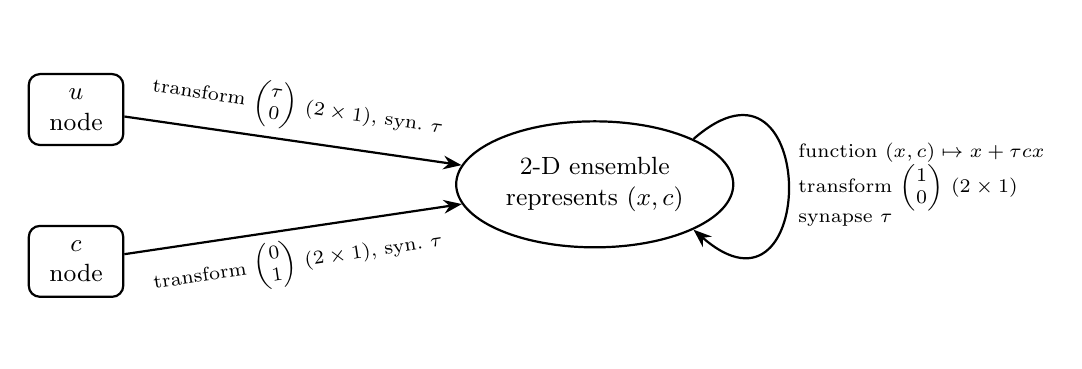
\begin{tikzpicture}[font=\small, node distance=1.5cm,
  box/.style={draw, thick, rounded corners, minimum height=0.9cm, minimum width=1.2cm, align=center}]
  \node[box] (u) {$u$\\node};
  \node[box, below=1.0cm of u] (c) {$c$\\node};
  \node[box, ellipse, right=4.2cm of u, yshift=-0.95cm, minimum width=2.6cm, minimum height=1.6cm] (e) {2-D ensemble\\represents $(x, c)$};
  \draw[-{Stealth}, thick] (u) -- node[above, sloped, font=\scriptsize] {transform $\begin{pmatrix}\tau\\0\end{pmatrix}$ ($2\times1$), syn.\ $\tau$} (e);
  \draw[-{Stealth}, thick] (c) -- node[below, sloped, font=\scriptsize] {transform $\begin{pmatrix}0\\1\end{pmatrix}$ ($2\times1$), syn.\ $\tau$} (e);
  \draw[-{Stealth}, thick] (e.north east) .. controls +(1.6,1.4) and +(1.6,-1.4) .. (e.south east)
    node[pos=0.5, right, font=\scriptsize, align=left] {function $(x, c) \mapsto x + \tau c x$\\transform $\begin{pmatrix}1\\0\end{pmatrix}$ ($2\times1$)\\synapse $\tau$};
\end{tikzpicture}
\end{center}
Dimension 2 has no recurrence, so it just follows the filtered $c$. Only dimension 1 is integrated.

\ans{Q2}
\begin{itemize}[leftmargin=1.2em]
\item $c = 0$: $x = t$ up to $0.5$, then it holds at $0.5$.
\item $c = -2$: $\dot x = -2x + 1$, so $x = \frac12(1 - e^{-2t})$, which is $\frac12(1 - e^{-1}) \approx 0.32$ at $t = 0.5$. After that it decays as $0.32e^{-2(t - 0.5)}$, with time constant $1/|c| = 0.5$ s.
\item $c = +1$: $\dot x = x + 1$, so $x = e^t - 1 \approx 0.65$ at $t = 0.5$. Then $0.65e^{t - 0.5}$ reaches $1$ at $t \approx 0.93$ s and saturates.
\end{itemize}
\begin{center}
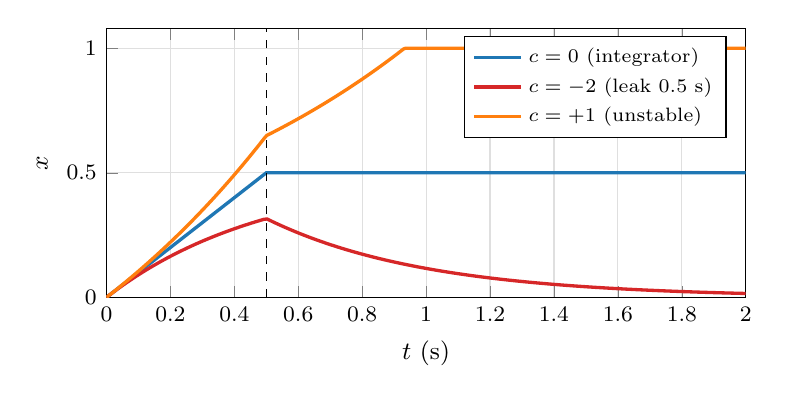
\begin{tikzpicture}
\begin{axis}[width=0.8\textwidth, height=5cm, xmin=0, xmax=2, ymin=0, ymax=1.08,
  xlabel={$t$ (s)}, ylabel={$x$}, legend pos=north east, legend cell align=left]
  \addplot[cA, very thick] coordinates {(0,0) (0.5,0.5) (2,0.5)};
  \addplot[cD, very thick, domain=0:2, samples=200] {(x<0.5)*0.5*(1-exp(-2*x)) + (x>=0.5)*0.31606*exp(-2*(x-0.5))};
  \addplot[cB, very thick, domain=0:2, samples=300] {min((x<0.5)*(exp(x)-1) + (x>=0.5)*0.64872*exp(x-0.5), 1)};
  \addplot[black, thin, dashed, forget plot] coordinates {(0.5,0) (0.5,1.08)};
  \legend{$c = 0$ (integrator), $c = -2$ (leak $0.5$ s), $c = +1$ (unstable)}
\end{axis}
\end{tikzpicture}
\end{center}
\begin{result}
$u$ in with $(\tau, 0)^\T$, $c$ in with $(0, 1)^\T$, recurrent $x + \tau cx$ into dimension 1. \ $c = 0$ holds $0.5$; $c = -2$ peaks at $0.32$ and decays with $0.5$ s; $c = +1$ runs to the radius.
\end{result}

%=====================================================================
\part*{Part C}
%=====================================================================

\ans{Q1}
$\tau\dot x = 2u - x - x = 2(u - x)$, so $\dot x = (u - x)/(\tau/2)$. This is a low-pass filter with steady state $u$ and time constant $\tau/2 = 10$ ms: $x = 1 - e^{-t/0.01}$, reaching $63\%$ at $10$ ms.
\begin{center}
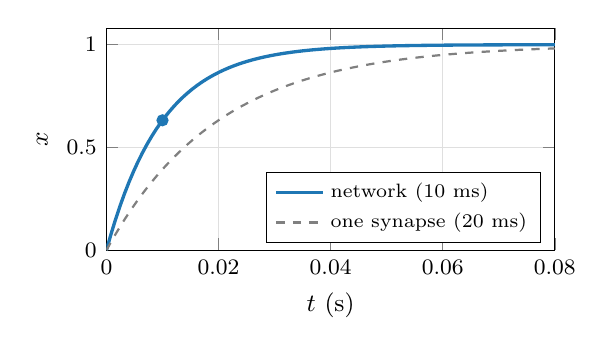
\begin{tikzpicture}
\begin{axis}[width=0.6\textwidth, height=4.4cm, xmin=0, xmax=0.08, ymin=0, ymax=1.08,
  xlabel={$t$ (s)}, ylabel={$x$}, legend pos=south east, legend cell align=left,
  scaled x ticks=false, xticklabel style={/pgf/number format/fixed}]
  \addplot[cA, very thick, domain=0:0.08, samples=100] {1-exp(-x/0.01)};
  \addplot[gray, dashed, thick, domain=0:0.08, samples=100] {1-exp(-x/0.02)};
  \legend{network ($10$ ms), one synapse ($20$ ms)}
  \addplot[only marks, mark=*, cA, forget plot] coordinates {(0.01,0.632)};
\end{axis}
\end{tikzpicture}
\end{center}

\ans{Q2}
$A = (0.9 - 1)/0.1 = -1\ \mathrm{s^{-1}}$ and $B = B'/\tau = 1$, so $\dot x = -x + u$: a leaky integrator with a $1$ s time constant. For $u = 0.8$ on $[0.2, 1.0)$: $x = 0.8(1 - e^{-(t - 0.2)})$, which is $0.8(1 - e^{-0.8}) \approx 0.44$ at $t = 1$, then $0.44e^{-(t - 1)}$. The ideal holds $0.64$.
\begin{center}
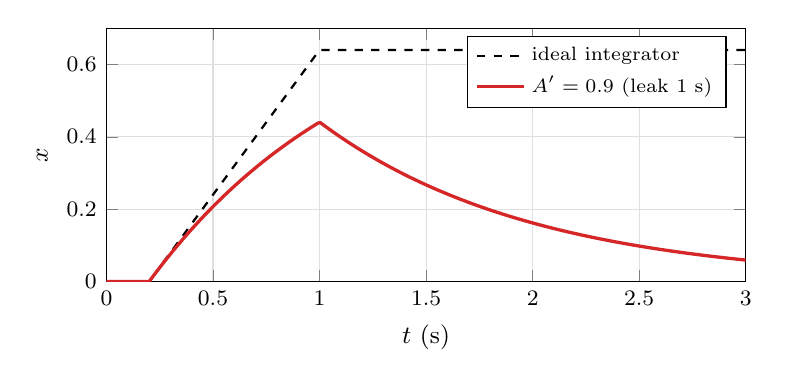
\begin{tikzpicture}
\begin{axis}[width=0.8\textwidth, height=4.8cm, xmin=0, xmax=3, ymin=0, ymax=0.7,
  xlabel={$t$ (s)}, ylabel={$x$}, legend pos=north east, legend cell align=left]
  \addplot[black, thick, dashed] coordinates {(0,0) (0.2,0) (1.0,0.64) (3,0.64)};
  \addplot[cD, very thick, domain=0:3, samples=300] {(x>=0.2)*(x<1)*0.8*(1-exp(-(x-0.2))) + (x>=1)*0.44067*exp(-(x-1))};
  \legend{ideal integrator, $A' = 0.9$ (leak $1$ s)}
\end{axis}
\end{tikzpicture}
\end{center}

\ans{Q3}
A synapse does not hold its value: it drifts toward whatever input it is given, losing its own value over a time of about $\tau$. Feeding the represented value back as input (the ``$+x$'') cancels that loss, so the loop holds its state and only changes when we add something extra. Multiplying the desired rate of change by $\tau$ converts it into the size of input the slow synapse needs in order to move at exactly that rate.

\end{document}
